\chapter{第3套试卷——参考答案与评分标准}

% 加载TikZ所需库（在主文档中可能未全部加载）
\usetikzlibrary{automata, positioning, arrows.meta}

% ======================================================================
\section{一、选择题（每题3分，共18分）}

\subsection*{参考答案与解析}

\begin{enumerate}[label=\arabic*., leftmargin=*]

\item \textbf{答案：D}

\noindent\textbf{解析：}
\begin{itemize}
  \item A项正确：CPLD确基于乘积项（Product Term）的与或阵列结构，适合实现宽输入的复杂组合逻辑（如地址译码）。
  \item B项正确：FPGA基于SRAM工艺的查找表（LUT），掉电后配置丢失，但可重复编程（在线重配置）。
  \item C项正确：FPGA的基本可编程逻辑单元是CLB（Configurable Logic Block），每个CLB包含若干个Slice，每个Slice包含LUT和Flip-Flop。
  \item D项\textbf{错误}：CPLD的延时是\textbf{可预测}的（由乘积项阵列的固定走线决定），这是CPLD的优势而非劣势。FPGA的延时反而不如CPLD可预测（取决于布局布线）。因此CPLD\underline{适合}时序要求严格的电路。
\end{itemize}

\medskip
\noindent\textbf{评分标准：}选D得3分；选其他不得分。

% ----------------------------------------------------------------------

\item \textbf{答案：B}

\noindent\textbf{解析：}FPGA中的查找表（LUT，Look-Up Table）本质上是一个小容量SRAM，存储了组合逻辑函数的真值表。一个$n$输入LUT可以实现任意$n$变量的组合逻辑函数（$2^{2^n}$种可能）。例如，4输入LUT可存储16位真值表数据，实现任意4输入1输出的组合逻辑。

\noindent\textbf{评分标准：}选B得3分；选其他不得分。

% ----------------------------------------------------------------------

\item \textbf{答案：B}

\noindent\textbf{解析：}VHDL中ENTITY（实体）声明用于描述设计单元与外部世界的接口，包括：
\begin{itemize}
  \item 端口名（Port Name）
  \item 端口方向（Mode：IN、OUT、INOUT、BUFFER）
  \item 端口数据类型（Type：如STD\_LOGIC、STD\_LOGIC\_VECTOR）
\end{itemize}
内部实现细节由ARCHITECTURE（结构体）描述。仿真激励由Testbench中的PROCESS生成。

\noindent\textbf{评分标准：}选B得3分；选其他不得分。

% ----------------------------------------------------------------------

\item \textbf{答案：C}

\noindent\textbf{解析：}Signal与Variable的核心区别：

\begin{table}[h]
\centering
\begin{tabular}{|l|c|c|}
\hline
\textbf{属性} & \textbf{SIGNAL（信号）} & \textbf{VARIABLE（变量）} \\
\hline
声明位置 & 可在ARCHITECTURE声明区（PROCESS外部）或PROCESS内部 & 只能在PROCESS或SUBPROGRAM内部 \\
\hline
赋值符号 & \texttt{<=} & \texttt{:=} \\
\hline
生效时刻 & 进程挂起时（或经过$\delta$延时） & 立即生效 \\
\hline
作用范围 & 全局（跨进程/模块） & 局部（仅所在进程/子程序内） \\
\hline
历史信息 & 可携带（如\texttt{s'event}） & 无 \\
\hline
\end{tabular}
\end{table}

\begin{itemize}
  \item A项错误：VARIABLE只能在PROCESS或子程序内部声明，不能在外部。
  \item B项错误：Signal赋值在进程结束时（或下一仿真周期）生效，不是立即；Variable才是立即生效。
  \item C项\textbf{正确}：Variable只能在PROCESS或SUBPROGRAM内部声明，使用\texttt{:=}赋值且立即生效。
  \item D项错误：Signal可以在ARCHITECTURE声明区（PROCESS外部）声明，也可以在多进程间共享。
\end{itemize}

\noindent\textbf{评分标准：}选C得3分；选其他不得分。

% ----------------------------------------------------------------------

\item \textbf{答案：B}

\noindent\textbf{解析：}PROCESS的敏感信号表（sensitivity list）定义了触发进程执行的信号集合。当敏感表中的任意信号发生事件（值发生变化）时，进程被激活并从上到下顺序执行一次。
\begin{itemize}
  \item 组合逻辑PROCESS：敏感表应包含所有输入信号，避免生成锁存器。
  \item 时序逻辑PROCESS：敏感表通常包含时钟信号（可能还有异步复位信号）。
\end{itemize}
注意：VHDL-2008支持\texttt{PROCESS(ALL)}，编译器自动推断所有读入信号加入敏感表。

\noindent\textbf{评分标准：}选B得3分；选其他不得分。

% ----------------------------------------------------------------------

\item \textbf{答案：C}

\noindent\textbf{解析：}
\begin{itemize}
  \item A项：\texttt{LIBRARY std; USE std.standard.ALL}——\texttt{std.standard}包定义了VHDL的基本类型（BIT、BOOLEAN、INTEGER等），但不含\texttt{STD\_LOGIC}。
  \item B项：\texttt{LIBRARY work; USE work.types.ALL}——work库是用户工作库，默认不存在\texttt{types}包，非标准定义。
  \item C项\textbf{正确}：\texttt{LIBRARY IEEE; USE IEEE.STD\_LOGIC\_1164.ALL}——IEEE 1164标准定义了九值逻辑系统，包括\texttt{STD\_LOGIC}和\texttt{STD\_LOGIC\_VECTOR}。
  \item D项：\texttt{LIBRARY IEEE; USE IEEE.NUMERIC\_STD.ALL}——该包定义了\texttt{UNSIGNED}和\texttt{SIGNED}算术类型及其运算，不含\texttt{STD\_LOGIC}定义。
\end{itemize}

\noindent\textbf{评分标准：}选C得3分；选其他不得分。

\end{enumerate}

% ======================================================================
\newpage
\section{二、填空题（每题3分，共12分）}

\subsection*{参考答案}

\begin{enumerate}[label=\arabic*., leftmargin=*]

\item \textbf{ENTITY}（实体）和\textbf{ARCHITECTURE}（结构体）

\noindent\textbf{解析：}VHDL中最基本的设计单元称为Design Entity（设计实体），由两部分构成：
\begin{itemize}
  \item \texttt{ENTITY}：声明设计的对外接口（端口名、方向、类型），即“黑盒”的外部视图。
  \item \texttt{ARCHITECTURE}：描述设计的内部功能实现（行为、数据流或结构描述），即“黑盒”的内部实现。
\end{itemize}
一个ENTITY可以对应多个ARCHITECTURE（如行为级和结构级），通过配置（CONFIGURATION）选择。

\noindent\textbf{评分标准：}每空1.5分，顺序可互换。填写中文“实体”和“结构体”也给分。

% ----------------------------------------------------------------------

\item \textbf{\texttt{<=}}、\textbf{\texttt{:=}}、\textbf{\texttt{\&}}

\noindent\textbf{解析：}
\begin{itemize}
  \item 信号赋值：\texttt{<=}（如 \texttt{q <= d;}）
  \item 变量赋值：\texttt{:=}（如 \texttt{tmp := a + b;}）
  \item 并置运算符：\texttt{\&}（如 \texttt{"1010" \& "0011"} 结果为 \texttt{"10100011"}）
\end{itemize}

\noindent\textbf{评分标准：}每空1分，符号必须完全正确。

% ----------------------------------------------------------------------

\item \textbf{IEEE.STD\_LOGIC\_1164} 和 \textbf{IEEE.NUMERIC\_STD}

\noindent\textbf{解析：}
\begin{itemize}
  \item \texttt{IEEE.STD\_LOGIC\_1164}包：定义了九值逻辑系统（\texttt{'U', 'X', '0', '1', 'Z', 'W', 'L', 'H', '-'}）以及\texttt{STD\_LOGIC}类型和\texttt{STD\_LOGIC\_VECTOR}类型及基本逻辑运算函数。
  \item \texttt{IEEE.NUMERIC\_STD}包：定义了\texttt{UNSIGNED}（无符号数）和\texttt{SIGNED}（有符号数补码）两种算术类型，提供了算术运算符（\texttt{+}、\texttt{-}、\texttt{*}等）、比较运算符和类型转换函数。
\end{itemize}
注意：\texttt{IEEE.STD\_LOGIC\_ARITH}（Synopsys）和\texttt{IEEE.STD\_LOGIC\_UNSIGNED}虽被一些旧教材使用，但已不被IEEE标准推荐。考试中应使用\texttt{IEEE.NUMERIC\_STD}。

\noindent\textbf{评分标准：}每空1.5分。注意包名的完整写法。

% ----------------------------------------------------------------------

\item \textbf{INOUT} 和 \textbf{BUFFER}

\noindent\textbf{解析：}VHDL的四种端口模式：

\begin{table}[h]
\centering
\begin{tabular}{|l|c|c|c|}
\hline
\textbf{端口模式} & \textbf{方向} & \textbf{可读（内部）} & \textbf{典型用途} \\
\hline
\texttt{IN}    & 输入   & 是 & 数据输入、控制信号 \\
\hline
\texttt{OUT}   & 输出   & 否（VHDL-93前） & 数据输出 \\
\hline
\texttt{INOUT} & 双向   & 是 & 数据总线（如I$^2$C的SDA） \\
\hline
\texttt{BUFFER}& 输出   & 是 & 计数器输出需内部回读时 \\
\hline
\end{tabular}
\end{table}

\noindent\textbf{补充说明：}VHDL-2008后\texttt{OUT}端口也可内部回读，但考试中以经典教材（VHDL-93）为准。

\noindent\textbf{评分标准：}每空1.5分，顺序可互换。

\end{enumerate}

% ======================================================================
\newpage
\section{三、程序改错题（共5分）}

\subsection*{参考答案}

\noindent 以下逐行指出错误并给出正确写法（找到任意5处错误即可得5分，全部6处写出不扣分）：

\medskip
\begin{framed}
\noindent\textbf{错误1（第1行）：}\texttt{LIBARY} 改为 \texttt{LIBRARY}

\textbf{错误2（第14行）：}\texttt{)} 后缺少分号，应改为 \texttt{);}

\textbf{错误3（第21行）：}\texttt{y <= d(2)} 后缺少分号，应改为 \texttt{y <= d(2);}

\textbf{错误4（第23行）：}\texttt{y = '0'} 赋值符号错误，应改为 \texttt{y <= '0';}

\textbf{错误5（第24行）：}\texttt{END CASE} 后缺少分号，应改为 \texttt{END CASE;}

\textbf{错误6（第26行）：}\texttt{END behavior} 结构体名称不匹配，应改为 \texttt{END behav;}
\end{framed}

\medskip
\subsection*{详细解析}

\begin{enumerate}[leftmargin=*]

\item \textbf{第1行：关键字拼写错误。}\texttt{LIBARY}缺少字母\texttt{R}，正确为\texttt{LIBRARY}。这是最基础的语法错误。

\item \textbf{第13--14行：PORT声明结束缺少分号。}ENTITY的PORT声明是一个完整的语句块，在闭合括号后必须加分号。修正后为：
\begin{lstlisting}
  PORT(
    d : IN STD_LOGIC_VECTOR(3 DOWNTO 0);
    s : IN STD_LOGIC_VECTOR(1 DOWNTO 0);
    y : OUT STD_LOGIC
  );
\end{lstlisting}

\item \textbf{第21行：CASE分支语句缺少分号。}\texttt{WHEN "10" => y <= d(2)}是一个完整的顺序语句，必须以分号结束。

\item \textbf{第23行：赋值符号错误。}在VHDL中，信号（SIGNAL）赋值必须使用\texttt{<=}，不能使用\texttt{=}（\texttt{=}仅用于相等比较和初始化赋值，不用于信号赋值语句）。这一错误极为常见，考查学生对两类赋值符号的掌握。

\item \textbf{第24行：END CASE缺少分号。}与\texttt{END IF}、\texttt{END PROCESS}类似，\texttt{END CASE}后面必须加分号表示该语句的结束。

\item \textbf{第26行：结构体名称不匹配。}ARCHITECTURE声明为\texttt{behav}，结尾必须对应\texttt{END behav}（或\texttt{END ARCHITECTURE behav}），不能写成\texttt{END behavior}。

\end{enumerate}

\subsection*{修正后的正确代码}

\begin{lstlisting}[language=VDL, numbers=left]
LIBRARY IEEE;                                    -- 修正1
USE IEEE.STD_LOGIC_1164.ALL;
ENTITY mux4to1 IS
  PORT(
    d : IN STD_LOGIC_VECTOR(3 DOWNTO 0);
    s : IN STD_LOGIC_VECTOR(1 DOWNTO 0);
    y : OUT STD_LOGIC
  );                                             -- 修正2
END mux4to1;
ARCHITECTURE behav OF mux4to1 IS
BEGIN
  PROCESS(d, s)
  BEGIN
    CASE s IS
      WHEN "00" => y <= d(0);
      WHEN "01" => y <= d(1);
      WHEN "10" => y <= d(2);                    -- 修正3
      WHEN "11" => y <= d(3);
      WHEN OTHERS => y <= '0';                   -- 修正4
    END CASE;                                    -- 修正5
  END PROCESS;
END behav;                                       -- 修正6
\end{lstlisting}

\noindent\textbf{评分标准：}
\begin{itemize}
  \item 正确找出并修正1处错误得1分，最多5分（满分）。
  \item 仅指出错误但未给出正确写法的，每处扣0.5分。
  \item 找出6处不扣分（第5处之后不再额外加分）。
  \item 错误位置的行号因原题行号可能随格式变化，只需指出类似于哪一行即可。
\end{itemize}

% ======================================================================
\newpage
\section{四、程序阅读分析题（共5分）}

\subsection*{参考答案}

\begin{enumerate}[label=(\arabic*), leftmargin=*]

\item （2分）\textbf{电路类型与基本功能：}

该程序描述的是\textbf{带异步复位的D触发器（D Flip-Flop with Asynchronous Reset）}。

基本功能：
\begin{itemize}
  \item 当复位信号\texttt{rst}为高电平（\texttt{'1'}）时，输出\texttt{q}被立即强制清零（\texttt{q <= '0'}），此操作与时钟无关。
  \item 当复位信号无效（\texttt{rst = '0'}）时，在时钟\texttt{clk}的上升沿，将输入数据\texttt{d}的值存入输出\texttt{q}，即\texttt{q(n+1) = d}（功能表：$Q_{n+1}=D$）。
\end{itemize}

\medskip
\noindent\textbf{评分标准：}准确回答“带异步复位的D触发器”得1分；正确描述功能得1分（提到异步复位清零+上升沿采数据）。

% ----------------------------------------------------------------------

\item （2分）\textbf{信号作用与复位类型判断：}

\begin{itemize}
  \item \texttt{clk}：时钟输入，上升沿有效。提供系统时序基准，控制数据采样的时刻。
  \item \texttt{d}：数据输入。在时钟上升沿时，该信号的值被采样并传递至输出\texttt{q}。
  \item \texttt{rst}：异步复位输入，高电平有效。当\texttt{rst='1'}时无论时钟为何状态，输出\texttt{q}立即被置为\texttt{'0'}。
  \item \texttt{q}：数据输出。输出当前存储的值（在复位时为\texttt{'0'}，否则为最近一次时钟上升沿采样到的\texttt{d}值）。
\end{itemize}

\noindent\textbf{该电路是异步复位。}理由：
\begin{enumerate}
  \item 从\textbf{代码结构}看：\texttt{rst}同时出现在PROCESS的敏感信号表中（\texttt{PROCESS(clk, rst)}）且\texttt{IF rst = '1'}优先级最高（写在\texttt{ELSIF rising\_edge(clk)}之前）。
  \item 从\textbf{行为特性}看：复位操作不依赖时钟沿——只要\texttt{rst}变为\texttt{'1'}，输出\texttt{q}立即被清零，无需等待时钟上升沿。这正是异步复位的本质特征。
  \item \textbf{补充对比}：若为同步复位，则敏感表中不会（也不需要）包含\texttt{rst}，且复位语句应放在时钟沿判断内部（如\texttt{IF rising\_edge(clk) THEN IF rst='1' THEN...}）。
\end{enumerate}

\medskip
\noindent\textbf{评分标准：}正确说明4个信号作用得1分（每个0.25分）；正确判断为异步复位并充分说明理由得1分。

% ----------------------------------------------------------------------

\item （1分）\textbf{\texttt{rising\_edge(clk)} 与 \texttt{clk'event AND clk='1'} 的比较：}

\textbf{功能上不完全相同。}

\begin{itemize}
  \item \texttt{rising\_edge(clk)} 是IEEE 1164定义的函数，其内部判断条件更为严格：
  \begin{itemize}
    \item 它要求信号发生了事件（\texttt{clk'event}），且当前值为\texttt{'1'}（\texttt{clk='1'}），\textbf{同时}上一值必须为\texttt{'0'}或\texttt{'L'}（弱低电平）。这保证了真正的“\texttt{'0'} $\rightarrow$ \texttt{'1'}上升沿”。
    \item 它不将\texttt{'Z'} $\rightarrow$ \texttt{'1'}、\texttt{'U'} $\rightarrow$ \texttt{'1'}等非正常跳变视为有效上升沿。
  \end{itemize}
  \item \texttt{clk'event AND clk='1'} 仅检查信号发生了事件且当前值为\texttt{'1'}，不检查上一值。这意味着从\texttt{'Z'}、\texttt{'U'}、\texttt{'X'}等状态跳变到\texttt{'1'}也会被当作有效时钟沿——这在实际硬件中是不合理的，且可能造成仿真与综合结果不一致。
  \item 对于\textbf{综合工具}而言，两者通常被映射为相同的硬件结构（上升沿触发的D触发器），因此在\textbf{综合后}\textbf{功能基本等价}。但在\textbf{仿真}中，\texttt{rising\_edge()}更加严谨，是推荐的标准写法。
\end{itemize}

\noindent\textbf{评分标准：}回答不完全相同并指出\texttt{rising\_edge()}更严格（检查从\texttt{'0'}或\texttt{'L'}跳变）得1分；仅回答“功能相同”不得分。

\end{enumerate}

% ======================================================================
\newpage
\section{五、综合设计题（共60分）}

% ----------------------------------------------------------------------
\subsection{设计题1：组合逻辑设计——8线-3线优先编码器（20分）}

\subsubsection*{(1) 真值表（8分）}

\noindent\textbf{说明：}输入\texttt{din(7$\sim$0)}低电平有效（0=请求），\texttt{din(7)}优先级最高，\texttt{din(0)}最低。表中“X”表示任意值（don’t care），\texttt{gs}为组选通信号。

\begin{table}[h]
\centering
\caption{8线-3线优先编码器真值表（低电平有效）}
\label{tab:priority-encoder}
\begin{tabular}{|c|c|c|c|c|c|c|c||c|c|c||c|}
\hline
\multicolumn{8}{|c||}{\textbf{输入 din(7$\sim$0)}} & \multicolumn{3}{c||}{\textbf{输出}} & \textbf{gs} \\
\hline
din7 & din6 & din5 & din4 & din3 & din2 & din1 & din0 & dout2 & dout1 & dout0 & gs \\
\hline
0 & X & X & X & X & X & X & X & 1 & 1 & 1 & 1 \\
\hline
1 & 0 & X & X & X & X & X & X & 1 & 1 & 0 & 1 \\
\hline
1 & 1 & 0 & X & X & X & X & X & 1 & 0 & 1 & 1 \\
\hline
1 & 1 & 1 & 0 & X & X & X & X & 1 & 0 & 0 & 1 \\
\hline
1 & 1 & 1 & 1 & 0 & X & X & X & 0 & 1 & 1 & 1 \\
\hline
1 & 1 & 1 & 1 & 1 & 0 & X & X & 0 & 1 & 0 & 1 \\
\hline
1 & 1 & 1 & 1 & 1 & 1 & 0 & X & 0 & 0 & 1 & 1 \\
\hline
1 & 1 & 1 & 1 & 1 & 1 & 1 & 0 & 0 & 0 & 0 & 1 \\
\hline
1 & 1 & 1 & 1 & 1 & 1 & 1 & 1 & 0 & 0 & 0 & 0 \\
\hline
\end{tabular}
\end{table}

\noindent\textbf{说明：}
\begin{itemize}
  \item 第1行：\texttt{din(7)=0}（第7路有效），无论其他输入为何，\texttt{dout="111"}（二进制7）。此时\texttt{gs='1'}，表示至少有一路输入有效。
  \item 第2行：\texttt{din(7)=1}（无效）且\texttt{din(6)=0}（有效），输出\texttt{"110"}（二进制6）。
  \item 依此类推，按优先级从高到低逐行判定。
  \item 最后一行：所有输入均为\texttt{'1'}（无效），\texttt{dout="000"}，\texttt{gs='0'}表示无请求。
\end{itemize}

\noindent\textbf{评分标准：}
\begin{itemize}
  \item 真值表格式正确（包含输入、输出、gs列）得2分。
  \item 正确体现“低电平有效”与优先级顺序（din7最高$\to$din0最低）得3分。
  \item 覆盖至少7种关键情况（包括无请求）得2分。
  \item 逻辑关系正确得1分。
\end{itemize}

% ----------------------------------------------------------------------

\subsubsection*{(2) 逻辑表达式（3分）}

\noindent 由真值表可导出各输出的逻辑表达式（卡诺图化简或直接推导）：

\medskip
\noindent\textbf{gs（组选通信号）：}
\[
\text{gs} = \overline{\text{din}(7) \cdot \text{din}(6) \cdot \text{din}(5) \cdot \text{din}(4) \cdot \text{din}(3) \cdot \text{din}(2) \cdot \text{din}(1) \cdot \text{din}(0)}
\]
即：\texttt{gs = '1'}当且仅当至少一个输入为\texttt{'0'}（低电平有效）。
等价写法：\texttt{gs = NOT (din(7) AND din(6) AND ... AND din(0))}。

\medskip
\noindent\textbf{dout(2)（最高位）：}
\[
\text{dout}(2) = \overline{\text{din}(7)} + \text{din}(7)\cdot\overline{\text{din}(6)} + \text{din}(7)\cdot\text{din}(6)\cdot\overline{\text{din}(5)} + \text{din}(7)\cdot\text{din}(6)\cdot\text{din}(5)\cdot\overline{\text{din}(4)}
\]
即：\texttt{dout(2)='1'}当最高优先级的有效输入位于\texttt{din(7,6,5,4)}之中（编号4$\sim$7）。

\medskip
\noindent\textbf{dout(1)：}
\[
\text{dout}(1) = \overline{\text{din}(7)} + \text{din}(7)\cdot\overline{\text{din}(6)} + \text{din}(7)\cdot\text{din}(6)\cdot\text{din}(5)\cdot\text{din}(4)\cdot\overline{\text{din}(3)} + \text{din}(7)\cdot\text{din}(6)\cdot\text{din}(5)\cdot\text{din}(4)\cdot\text{din}(3)\cdot\overline{\text{din}(2)}
\]
即：\texttt{dout(1)='1'}当最高优先级的有效输入位于\texttt{din(7,6,3,2)}之中（编号的二进制中间位为1）。

\medskip
\noindent\textbf{dout(0)：}
\[
\text{dout}(0) = \overline{\text{din}(7)} + \text{din}(7)\cdot\text{din}(6)\cdot\overline{\text{din}(5)} + \text{din}(7)\cdot\text{din}(6)\cdot\text{din}(5)\cdot\text{din}(4)\cdot\overline{\text{din}(3)} + \text{din}(7)\cdot\text{din}(6)\cdot\text{din}(5)\cdot\text{din}(4)\cdot\text{din}(3)\cdot\text{din}(2)\cdot\overline{\text{din}(1)}
\]
即：\texttt{dout(0)='1'}当最高优先级的有效输入位于\texttt{din(7,5,3,1)}之中（编号的二进制最低位为1）。

\medskip
\noindent\textbf{评分标准：}
\begin{itemize}
  \item gs表达式正确得1分。
  \item dout(2)、dout(1)、dout(0)表达式各0.5分，合计1.5分。
  \item 逻辑关系正确即可得满分，表达式的等价形式（如\texttt{NOR-NAND}形式）也给分，共0.5分。
\end{itemize}

% ----------------------------------------------------------------------

\subsubsection*{(3) VHDL代码——条件信号赋值语句实现（9分）}

\noindent\textbf{方案一：WHEN-ELSE语句实现（推荐，符合优先级编码逻辑）}

\begin{lstlisting}[language=VDL, numbers=left]
LIBRARY IEEE;
USE IEEE.STD_LOGIC_1164.ALL;
USE IEEE.NUMERIC_STD.ALL;       -- 若不需要算术运算可省略

ENTITY priority_encoder_83 IS
  PORT(
    din  : IN  STD_LOGIC_VECTOR(7 DOWNTO 0);  -- 低电平有效
    dout : OUT STD_LOGIC_VECTOR(2 DOWNTO 0);  -- 二进制编码输出
    gs   : OUT STD_LOGIC                      -- 组选通信号
  );
END priority_encoder_83;

ARCHITECTURE behav OF priority_encoder_83 IS
BEGIN

  -- 条件信号赋值：从高优先级到低优先级依次判断
  dout <= "111" WHEN din(7) = '0' ELSE    -- 优先级7（最高）
          "110" WHEN din(6) = '0' ELSE    -- 优先级6
          "101" WHEN din(5) = '0' ELSE    -- 优先级5
          "100" WHEN din(4) = '0' ELSE    -- 优先级4
          "011" WHEN din(3) = '0' ELSE    -- 优先级3
          "010" WHEN din(2) = '0' ELSE    -- 优先级2
          "001" WHEN din(1) = '0' ELSE    -- 优先级1
          "000";                           -- 优先级0（最低）或无请求

  -- 组选通信号：当任意输入有效时，gs = '1'
  gs <= '0' WHEN din = "11111111" ELSE '1';

END behav;
\end{lstlisting}

\medskip
\noindent\textbf{方案二：WITH-SELECT-WHEN语句实现}

\begin{lstlisting}[language=VDL, numbers=left]
ARCHITECTURE dataflow OF priority_encoder_83 IS
BEGIN
  -- 使用WITH-SELECT，需枚举所有din取值组合（部分简化为含don't care的写法）
  -- 注意：WITH-SELECT中WHEN的选择值必须互斥且完备
  WITH din SELECT
    dout <= "111" WHEN "0-------",   -- din(7)=0
            "110" WHEN "10------",   -- din(7)=1, din(6)=0
            "101" WHEN "110-----",   -- din(7..6)=11, din(5)=0
            "100" WHEN "1110----",   -- din(7..5)=111, din(4)=0
            "011" WHEN "11110---",   -- ...
            "010" WHEN "111110--",
            "001" WHEN "1111110-",
            "000" WHEN "11111110",
            "000" WHEN OTHERS;       -- 全1或全0等

  gs <= '0' WHEN din = "11111111" ELSE '1';
END dataflow;
\end{lstlisting}

\noindent\textbf{说明：}方案二中的don't care写法（如\texttt{"0-------"}）在VHDL-2008及部分综合工具中支持，但在严格VHDL-93/87中可能不被接受。考试中\textbf{推荐使用方案一（WHEN-ELSE）}，清晰且可综合性强。

\medskip
\noindent\textbf{评分标准：}
\begin{itemize}
  \item ENTITY声明正确（含端口名、方向、数据类型）得2分。
  \item 库和包引用正确得1分。
  \item 条件信号赋值语句使用正确（WHEN-ELSE或WITH-SELECT）得2分。
  \item 优先级顺序正确（从din(7)到din(0)依次判断）得2分。
  \item gs信号逻辑正确得1分。
  \item 代码格式规范、无语法错误得1分。
\end{itemize}

% ======================================================================
\newpage
\subsection{设计题2：时序逻辑设计——模10 BCD计数器（20分）}

\subsubsection*{(1) 状态转换图（4分）}

\begin{figure}[h]
\centering
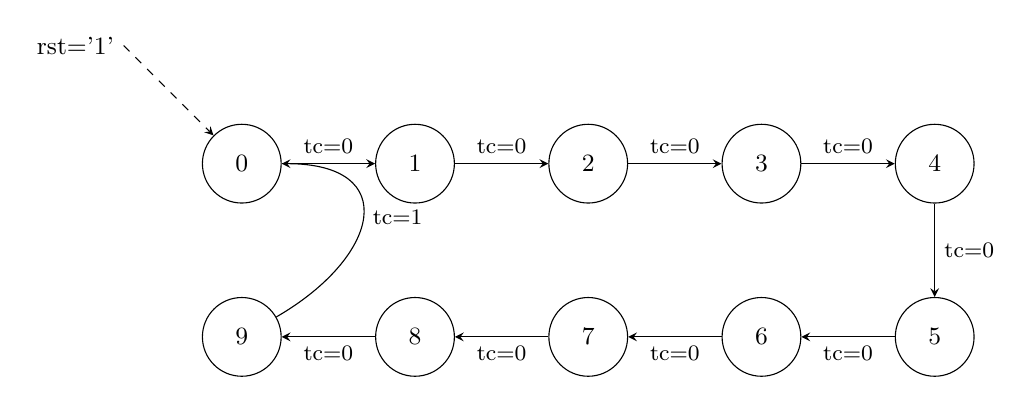
\begin{tikzpicture}[
    ->,
    >=stealth,
    node distance=2.2cm and 3cm,
    state/.style={circle, draw, minimum size=1.0cm, inner sep=0pt, font=\small}
  ]

  % 10个状态节点
  \node[state] (s0) {0};
  \node[state] (s1) [right of=s0] {1};
  \node[state] (s2) [right of=s1] {2};
  \node[state] (s3) [right of=s2] {3};
  \node[state] (s4) [right of=s3] {4};
  \node[state] (s5) [below of=s4] {5};
  \node[state] (s6) [left of=s5] {6};
  \node[state] (s7) [left of=s6] {7};
  \node[state] (s8) [left of=s7] {8};
  \node[state] (s9) [left of=s8] {9};

  % 转换箭头
  \draw (s0) -- (s1) node[midway, above] {\footnotesize tc=0};
  \draw (s1) -- (s2) node[midway, above] {\footnotesize tc=0};
  \draw (s2) -- (s3) node[midway, above] {\footnotesize tc=0};
  \draw (s3) -- (s4) node[midway, above] {\footnotesize tc=0};
  \draw (s4) -- (s5) node[midway, right] {\footnotesize tc=0};
  \draw (s5) -- (s6) node[midway, below] {\footnotesize tc=0};
  \draw (s6) -- (s7) node[midway, below] {\footnotesize tc=0};
  \draw (s7) -- (s8) node[midway, below] {\footnotesize tc=0};
  \draw (s8) -- (s9) node[midway, below] {\footnotesize tc=0};

  % 从9回到0的弧线（产生tc=1脉冲）
  \draw[->] (s9) to[out=30, in=0, looseness=2]
        node[midway, right, font=\footnotesize] {tc=1} (s0);

  % 复位箭头（所有状态均可复位至0）
  \draw[->, dashed] (-1.5,1.5) node[left, font=\small] {rst='1'} -- (s0);

\end{tikzpicture}
\caption{模10 BCD计数器状态转换图}
\label{fig:bcd-counter}
\end{figure}

\noindent\textbf{说明：}
\begin{itemize}
  \item 计数范围：0 $\to$ 1 $\to$ 2 $\to$ \dots $\to$ 9 $\to$ 0（循环），每个时钟上升沿计数值+1。
  \item 除9$\to$0转换时\texttt{tc='1'}外，其余转换\texttt{tc='0'}。
  \item 复位信号\texttt{rst='1'}时（同步复位，在时钟上升沿采样），计数器回到0状态。
\end{itemize}

\noindent\textbf{评分标准：}
\begin{itemize}
  \item 状态节点完整（0$\sim$9，10个状态）得1分。
  \item 状态转换方向正确得1分。
  \item 转换条件标注清晰得1分。
  \item 复位关系和tc=1的跳变标注正确得1分。
\end{itemize}

% ----------------------------------------------------------------------

\subsubsection*{(2) tc信号产生逻辑（3分）}

\noindent\textbf{tc（Terminal Count，进位/终端计数）信号：}

\texttt{tc}是一个组合逻辑输出，仅当\textbf{当前计数值为9}\texttt{(count = "1001")}时输出高电平（\texttt{'1'}），其余计数值时输出低电平（\texttt{'0'}）。

\medskip
\noindent\textbf{逻辑表达式：}
\[
\text{tc} = \text{count}(3) \cdot \overline{\text{count}(2)} \cdot \overline{\text{count}(1)} \cdot \text{count}(0)
\]
即：\texttt{tc = count(3) AND (NOT count(2)) AND (NOT count(1)) AND count(0)}。

等价于：\texttt{tc = '1' WHEN count = "1001" ELSE '0';}

\medskip
\noindent\textbf{工作原理：}
\begin{itemize}
  \item 当计数器处于状态9（\texttt{count="1001"}）时，\texttt{tc='1'}，持续一个完整的时钟周期。
  \item 在下一个时钟上升沿，计数器从9跳变到0（若\texttt{rst='0'}），此时\texttt{tc}由\texttt{'1'}变为\texttt{'0'}，形成一个\textbf{高电平脉冲}（宽度为一个时钟周期）。
  \item 该脉冲可用于级联多级计数器时的进位使能，或作为状态机的外部触发信号。
\end{itemize}

\noindent\textbf{注意：}虽然\texttt{tc}从9$\to$0的转换中看似产生了“脉冲”，实际上\texttt{tc}是\textbf{纯组合逻辑}（仅取决于当前计数值），其脉宽为一个时钟周期是因为计数值在该周期内保持为9。

\medskip
\noindent\textbf{评分标准：}
\begin{itemize}
  \item 正确说明tc='1'的条件（count=9）得1分。
  \item 给出逻辑表达式或等效描述得1分。
  \item 说明tc在9$\to$0时产生一个时钟周期脉冲得1分。
\end{itemize}

% ----------------------------------------------------------------------

\subsubsection*{(3) VHDL代码——含内部信号count（13分）}

\begin{lstlisting}[language=VDL, numbers=left]
LIBRARY IEEE;
USE IEEE.STD_LOGIC_1164.ALL;
USE IEEE.NUMERIC_STD.ALL;

ENTITY bcd_counter_mod10 IS
  PORT(
    clk : IN  STD_LOGIC;                    -- 时钟
    rst : IN  STD_LOGIC;                    -- 同步复位，高有效
    q   : OUT STD_LOGIC_VECTOR(3 DOWNTO 0); -- BCD计数值输出
    tc  : OUT STD_LOGIC                     -- 终端计数（进位）输出
  );
END bcd_counter_mod10;

ARCHITECTURE behav OF bcd_counter_mod10 IS

  -- 内部信号：保存当前计数值
  SIGNAL count : UNSIGNED(3 DOWNTO 0) := (OTHERS => '0');
    -- 也可用 STD_LOGIC_VECTOR 或 INTEGER RANGE 0 TO 9

BEGIN

  -- 时序进程：计数逻辑（同步复位）
  PROCESS(clk)
  BEGIN
    IF rising_edge(clk) THEN
      IF rst = '1' THEN                    -- 同步复位
        count <= (OTHERS => '0');          -- 计数值清零
      ELSE
        IF count = 9 THEN                  -- 到达最大值9
          count <= (OTHERS => '0');        -- 回到0
        ELSE
          count <= count + 1;              -- 否则+1
        END IF;
      END IF;
    END IF;
  END PROCESS;

  -- 输出赋值：内部count信号输出到端口 & 产生tc信号
  q  <= STD_LOGIC_VECTOR(count);           -- 类型转换（若count为UNSIGNED）
  tc <= '1' WHEN count = 9 ELSE '0';       -- 计数值为9时tc=1

END behav;
\end{lstlisting}

\medskip
\noindent\textbf{代码说明：}
\begin{enumerate}
  \item \textbf{内部信号count}：使用\texttt{UNSIGNED}类型存储当前计数值，初始化为0。
  \item \textbf{同步复位}：\texttt{IF rst = '1'}写在\texttt{IF rising\_edge(clk)}内部，复位操作在时钟上升沿采样。敏感表中仅含\texttt{clk}，不含\texttt{rst}。
  \item \textbf{计数逻辑}：\texttt{count = 9}时回0，否则\texttt{count + 1}。
  \item \textbf{tc输出}：条件信号赋值（组合逻辑），\texttt{count=9}时\texttt{tc='1'}，否则\texttt{tc='0'}。
  \item \textbf{类型转换}：\texttt{STD\_LOGIC\_VECTOR(count)}将UNSIGNED类型转换为STD\_LOGIC\_VECTOR类型输出。
\end{enumerate}

\medskip
\noindent\textbf{评分标准：}
\begin{itemize}
  \item ENTITY端口声明正确得2分。
  \item 库引用正确（IEEE + NUMERIC\_STD）得1分。
  \item 内部信号count声明正确得1分。
  \item 复位为同步复位（写在IF rising\_edge(clk)内部）得2分。
  \item 计数逻辑正确（0$\to$9$\to$0循环）得2分。
  \item tc信号组合逻辑正确得2分。
  \item 输出q与内部count信号连接正确得1分。
  \item PROCESS语法正确、代码格式规范得2分。
\end{itemize}

% ======================================================================
\newpage
\subsection{设计题3：状态机设计——Moore型“101”序列检测器（20分）}

\subsubsection*{(1) 状态转换图（6分）}

\noindent\textbf{状态定义：}
\begin{itemize}
  \item \textbf{S0}：初始/复位状态，尚未检测到有效位。输出\texttt{z = '0'}。
  \item \textbf{S1}：已检测到序列第1位\texttt{'1'}。输出\texttt{z = '0'}。
  \item \textbf{S2}：已检测到序列\texttt{'10'}。输出\texttt{z = '0'}。
  \item \textbf{S3}：已检测到完整序列\texttt{'101'}。输出\texttt{z = '1'}。
\end{itemize}

\noindent\textbf{状态编码方案：}使用用户自定义枚举类型，由综合工具自动分配编码（通常为二进制编码：S0="00", S1="01", S2="10", S3="11"），也可手动指定（如One-Hot编码）。

\begin{figure}[h]
\centering
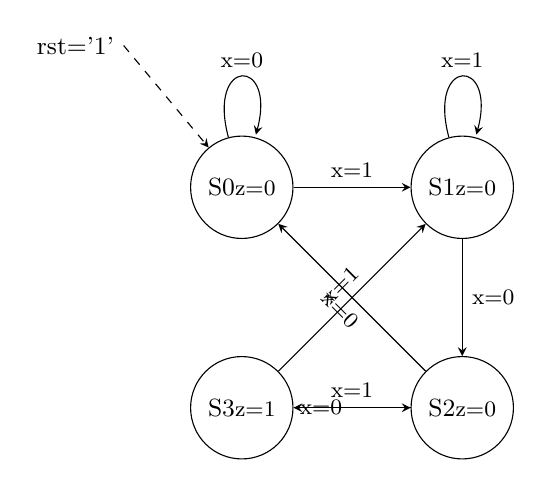
\begin{tikzpicture}[
    ->,
    >=stealth,
    auto,
    node distance=2.8cm and 4cm,
    state/.style={circle, draw, minimum size=1.3cm, inner sep=0pt, font=\small}
  ]

  % 4个状态节点
  \node[state] (s0)                    {S0\\\footnotesize z=0};
  \node[state] (s1) [right of=s0]     {S1\\\footnotesize z=0};
  \node[state] (s2) [below of=s1]     {S2\\\footnotesize z=0};
  \node[state] (s3) [below of=s0]     {S3\\\footnotesize z=1};

  % S0转移
  \draw (s0) edge[loop above]  node[font=\footnotesize] {x=0} (s0);
  \draw (s0) -- (s1) node[midway, above, font=\footnotesize] {x=1};

  % S1转移
  \draw (s1) edge[loop above]  node[font=\footnotesize] {x=1} (s1);
  \draw (s1) -- (s2) node[midway, right, font=\footnotesize] {x=0};

  % S2转移
  \draw (s2) -- (s3) node[midway, above, font=\footnotesize] {x=1};
  \draw (s2) -- (s0) node[midway, below, font=\footnotesize, sloped] {x=0};

  % S3转移（重叠检测的关键）
  \draw (s3) -- (s1) node[midway, left, font=\footnotesize, sloped, above] {x=1};
  \draw (s3) -- (s2) node[midway, left, font=\footnotesize] {x=0};

  % 异步复位箭头
  \draw[->, dashed] (-1.5, 1.8) node[left, font=\small] {rst='1'} -- (s0);

\end{tikzpicture}
\caption{Moore型“101”序列检测器状态转换图（重叠检测）}
\label{fig:moor-fsm}
\end{figure}

\noindent\textbf{重叠检测示例：}输入序列\texttt{"10101"}：
\begin{itemize}
  \item 时刻1: x=1, S0$\to$S1, z=0
  \item 时刻2: x=0, S1$\to$S2, z=0
  \item 时刻3: x=1, S2$\to$S3, z=1（第1次检测）
  \item 时刻4: x=0, S3$\to$S2, z=0（重叠：S3检测到序列后，x=0将状态引回S2而非S0）
  \item 时刻5: x=1, S2$\to$S3, z=1（第2次检测）
\end{itemize}

\noindent\textbf{评分标准：}
\begin{itemize}
  \item 4个状态定义正确（S0初始、S1得1、S2得10、S3得101）得2分。
  \item 状态输出正确（仅S3的z=1，其他z=0）得1分。
  \item 状态转换条件标注完整正确得1分。
  \item 正确体现重叠检测（S3出x=1$\to$S1, x=0$\to$S2）得1分。
  \item 异步复位箭头标注正确得0.5分。
  \item 整体图清晰、标注规范得0.5分。
\end{itemize}

% ----------------------------------------------------------------------

\subsubsection*{(2) 状态转换表（4分）}

\begin{table}[h]
\centering
\caption{Moore型“101”序列检测器状态转换表}
\label{tab:fsm-table}
\begin{tabular}{|c|c||c|c|}
\hline
\textbf{当前状态} & \textbf{输入 x} & \textbf{次态} & \textbf{输出 z} \\
\hline
S0 & 0 & S0 & 0 \\
S0 & 1 & S1 & 0 \\
\hline
S1 & 0 & S2 & 0 \\
S1 & 1 & S1 & 0 \\
\hline
S2 & 0 & S0 & 0 \\
S2 & 1 & S3 & 0 \\
\hline
S3 & 0 & S2 & 1 \\
S3 & 1 & S1 & 1 \\
\hline
\end{tabular}
\end{table}

\noindent\textbf{说明：}
\begin{itemize}
  \item 当前状态S3且输出z=1时：若x=0，次态跳转至S2（为序列“10”的下一可能“101”做准备，重叠）；若x=1，次态跳转至S1（当前“1”可作为下一序列的起始位）。
  \item Moore型状态机：输出z仅依赖于当前状态，与输入x无关。故S0$\sim$S2输出恒为0，S3输出恒为1。
\end{itemize}

\noindent\textbf{评分标准：}
\begin{itemize}
  \item 状态转换表格式完整（当前状态、输入、次态、输出四列）得1分。
  \item 8行转换关系全部正确得2分（每错一行扣0.25分，直至0分）。
  \item 输出z仅取决于当前状态（Moore型特征）得1分。
\end{itemize}

% ----------------------------------------------------------------------

\subsubsection*{(3) VHDL代码——三进程描述风格（10分）}

\noindent\textbf{代码特点：}
\begin{itemize}
  \item 用户自定义枚举类型\texttt{state\_type}定义状态。
  \item \textbf{三进程描述风格：}进程1为时序状态寄存器（含异步复位），进程2为组合次态逻辑，进程3为组合输出逻辑。清晰分离三大功能模块。
  \item 异步复位：\texttt{rst}既出现在敏感表中，又作为时序进程中\texttt{IF}判断的最高优先级条件。
\end{itemize}

\begin{lstlisting}[language=VDL, numbers=left]
LIBRARY IEEE;
USE IEEE.STD_LOGIC_1164.ALL;

ENTITY seq_detector_101 IS
  PORT(
    clk : IN  STD_LOGIC;      -- 时钟
    rst : IN  STD_LOGIC;      -- 异步复位，高电平有效
    x   : IN  STD_LOGIC;      -- 串行数据输入
    z   : OUT STD_LOGIC       -- 检测结果输出
  );
END seq_detector_101;

ARCHITECTURE moore OF seq_detector_101 IS

  -- 用户自定义枚举类型：4个状态
  TYPE state_type IS (S0, S1, S2, S3);

  -- 状态信号（当前状态和次态）
  SIGNAL current_state : state_type;
  SIGNAL next_state    : state_type;

BEGIN

  -- ==========================================================
  -- 进程1：时序进程——状态寄存器（含异步复位）
  -- ==========================================================
  PROCESS(clk, rst)
  BEGIN
    IF rst = '1' THEN                    -- 异步复位，最高优先级
      current_state <= S0;               -- 复位到初始状态S0
    ELSIF rising_edge(clk) THEN          -- 时钟上升沿
      current_state <= next_state;       -- 状态更新
    END IF;
  END PROCESS;

  -- ==========================================================
  -- 进程2：组合进程——次态逻辑
  -- ==========================================================
  PROCESS(current_state, x)
  BEGIN
    -- 默认赋值（避免锁存器）
    next_state <= S0;

    CASE current_state IS

      WHEN S0 =>                         -- 初始状态
        IF x = '1' THEN
          next_state <= S1;              -- 检测到第1位'1'
        ELSE
          next_state <= S0;              -- 保持等待
        END IF;

      WHEN S1 =>                         -- 已检测到"1"
        IF x = '0' THEN
          next_state <= S2;              -- 检测到"10"
        ELSE
          next_state <= S1;              -- 仍是'1'，等待'0'
        END IF;

      WHEN S2 =>                         -- 已检测到"10"
        IF x = '1' THEN
          next_state <= S3;              -- 检测到"101"，进入成功状态
        ELSE
          next_state <= S0;              -- 断序，回到初始
        END IF;

      WHEN S3 =>                         -- 已检测到"101"（成功）
        IF x = '1' THEN
          next_state <= S1;              -- 重叠：当前'1'作为新序列起始
        ELSE
          next_state <= S2;              -- 重叠：当前'0'延续为"10"的第二位
        END IF;

      WHEN OTHERS =>
        next_state <= S0;                -- 安全处理

    END CASE;
  END PROCESS;

  -- ==========================================================
  -- 进程3：组合进程——输出逻辑（Moore型）
  -- ==========================================================
  PROCESS(current_state)
  BEGIN
    -- Moore型：输出仅取决于当前状态
    CASE current_state IS
      WHEN S3 =>
        z <= '1';                        -- 仅在S3状态输出1
      WHEN OTHERS =>
        z <= '0';                        -- 其他状态输出0
    END CASE;
  END PROCESS;

END moore;
\end{lstlisting}

\medskip
\noindent\textbf{三进程风格说明：}
\begin{enumerate}
  \item \textbf{进程1（时序——状态寄存器）：}负责在时钟上升沿（或异步复位）时将次态值打入当前状态寄存器。敏感表含\texttt{clk}和\texttt{rst}。异步复位判断的优先级最高。
  \item \textbf{进程2（组合——次态逻辑）：}纯组合逻辑，根据当前状态和输入x计算次态。敏感表必须包含所有输入信号（\texttt{current\_state, x}），且建议添加默认赋值（如\texttt{next\_state <= S0}）以避免推断锁存器。
  \item \textbf{进程3（组合——输出逻辑）：}纯组合逻辑，根据当前状态产生输出z。Moore型FSM中，输出与输入x无关，仅取决于当前状态。
\end{enumerate}

\noindent\textbf{评分标准：}
\begin{itemize}
  \item ENTITY声明正确得1分。
  \item 枚举类型\texttt{state\_type}定义正确得1分。
  \item 异步复位实现正确（敏感表含rst + IF rst优先 + 时序进程）得2分。
  \item 次态逻辑完全正确（含重叠检测的S3出转移）得2分。
  \item Moore型输出逻辑正确（z仅取决于current\_state）得1分。
  \item 三进程风格清晰、结构规范得1分。
  \item 组合进程敏感表完整、无锁存器隐患得1分。
  \item 代码整体格式整洁、注释合理得1分。
\end{itemize}

% ======================================================================
\newpage
\section*{本套试卷总分汇总}

\begin{table}[h]
\centering
\begin{tabular}{|l|c|}
\hline
\textbf{题型} & \textbf{满分} \\
\hline
一、选择题（6$\times$3） & 18分 \\
\hline
二、填空题（4$\times$3） & 12分 \\
\hline
三、程序改错题 & 5分 \\
\hline
四、程序阅读分析题 & 5分 \\
\hline
五、综合设计题 & 60分 \\
\quad 设计题1：8线-3线优先编码器 & 20分 \\
\quad 设计题2：模10 BCD计数器 & 20分 \\
\quad 设计题3：Moore型序列检测器 & 20分 \\
\hline
\textbf{合计} & \textbf{100分} \\
\hline
\end{tabular}
\end{table}

\endinput
